\documentclass{beamer}

\usepackage{../personal-packages/mathy-presentation}

\title{On sentences}
\subtitle{This is a sentence.}
\author{Thomas Schouten}
\date{\today}

\begin{document}

    \frame{\titlepage}

    % Possibilities for framefont: \tiny, \scriptsize, \footnotesize, \small, \normalsize, \large, \Large, \LARGE, \huge, \Huge

%    \begin{framefont}{\normalsize}
%        \begin{frame}
%            \frametitle{}
%
%        \end{frame}
%    \end{framefont}

    \begin{framefont}{\small}
        \begin{frame}
            \frametitle{`Has eighteen letters' does.}
            If the meanings of `true' and `false' were switched, then this sentence wouldn't be false.
            \begin{itemize}
                \item This sentence contains only one nonstandard English flutzpah.
                \item No language can express every thought unambiguously, least of all this one.
                \item You have, of course, just begun reading the sentence that you just finished reading.
                \item Although this sentence begins with the word `because', it is false.
                \item ``I am not the subject of this sentence.''
                \item I am the thought you are now thinking.
                \item Thit sentence is not self-referential because ``thit'' is not a word.
                \item When you are not looking at it, this sentence is in Spanish.
                \item The sentence now before your eyes spent a month in Hungarian last year and was only recently translated back into English.
                \item If this sentence didn't exist, somebody would have invented it.
                If I had finished this sentence,
            \end{itemize}
        \end{frame}
    \end{framefont}

    \begin{framefont}{\large}
        \begin{frame}
            \frametitle{The Hofstadter autobiography }

            I'm So Meta, Even This Acronym


            {\tiny by Randall Munroe.
             ``This is the reference implementation of the self-referential joke''}

            \vspace*{1cm}
            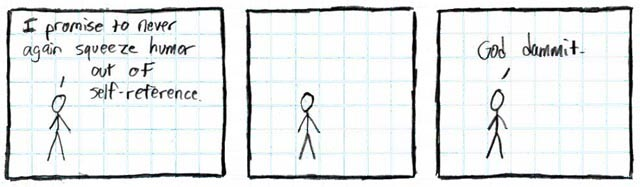
\includegraphics[width=\textwidth]{../src/png.jpg}

            {\tiny by Randall Munroe. ``I think about self-reference a lot. Example: this comment.''}
        \end{frame}
    \end{framefont}

\end{document}